% !Mode:: "TeX:UTF-8"

\begin{frame}{第十四讲、方向导数与梯度、Hessian矩阵及Taylor公式}
	\linespread{1.5}
	\begin{enumerate}
	  \item {\bf 内容与要求}{\b (\S10.4)}
	  \begin{itemize}
	    \item 理解方向导数与梯度的概念
	    \item 掌握方向导数与梯度的性质及应用
	    \item 理解Hessian矩阵及多元Taylor公式
	  \vspace{1em}
	  \end{itemize}
	  \item {\bf  课后作业:}
	  \begin{itemize}
	    \item {\b 习题10.4:1,3,4,5,7,8,9,11,15}
	  \end{itemize}
	\end{enumerate}
\end{frame}

\section{方向导数}

\begin{frame}{多元函数偏导数的几何意义}
	\linespread{1.2}\pause 
	设$z=f(x,y)$在$P(x_0,y_0)$可微,则$f\,'_x(x_0,y_0)$即为
	\begin{itemize}
	  \item 空间曲线
	  $$C:\left\{\begin{array}{l}
	  	z=f(x,y)\\ y=y_0
	  \end{array}\right.$$
	  在$(x_0,y_0,f(x_0,y_0))$的切线关于$x$的斜率\pause 
	  \item {\b 曲面在$(x_0,y_0,f(x_0,y_0))$处沿$x$轴方向的切线斜率}
	\end{itemize}
	\bigskip\pause 
	\centerline{\ba{如何定义/计算曲面在$P$点处沿任意方向的切线斜率?}}
\end{frame}

\begin{frame}{方向导数}
	\linespread{1.2}
	\centerline{\ba{如何定义/计算曲面在某点处沿任意方向的切线斜率?}}
	
	\bigskip\pause 
	{\bf 已知:}\pause 
	\begin{enumerate}
	  \item 曲面$S:z=f(x,y)$\pause 
	  \item $P(x_0,y_0,z_0)\in S$\pause 
	  \item $xOy$平面内的二维向量$\bm{u}$\pause 
	\end{enumerate}
	\bigskip
	{\bf 求:}$z$在$P$处沿方向$\bm{u}$的变化率(斜率)
\end{frame}

\begin{frame}{方向导数}
	\linespread{1.2}
	$z$在$P$处沿方向$\bm{u}$的变化率(斜率)\pause 
	$$k=\lim\limits_{h\to 0}\df{z(Q)-z(P)}{h}$$
	\vspace{-1em}\pause 
	\begin{block}{{\bf 定义}\hfill}
		{\bb $z=f(x,y)$在$(x_0,y_0)$沿$\bm{u}=(\cos\alpha,\cos\beta)$的方向导数:}\pause 
		%\vspace{-3ex}
		$$\alert{D_{\bm{u}}f(x_0,y_0)=\lim\limits_{h\to 0}
		\df{f(x_0+h\cos\alpha,y_0+h\cos\beta)-f(x_0,y_0)}{h}}$$
	\end{block}\pause 
	{\bf 注:}$D_{\bm{i}}f(x_0,y_0)=f\,'_x(x_0,y_0),\;\pause 
	D_{\bm{j}}f(x_0,y_0)=f\,'_y(x_0,y_0)$
\end{frame}

\begin{frame}{方向导数的计算}
	\linespread{1.2}\pause 
	\begin{block}{{\bf 定理10.4.1}\hfill}
		设函数$z=f(x,y)$在$P(x_0,y_0)$处可微,\pause 则在该点处沿任意方向
		$\bm{u}$的方向导数存在,\pause 且
		$$D_{\bm{u}}f(x_0,y_0) =f\,'_x(x_0,y_0)\cos\alpha+f\,'_y(x_0,y_0)\cos\beta$$
		其中$\cos\alpha,\cos\beta$为$\bm{u}$的方向余弦。
	\end{block}
\end{frame}

\begin{frame}
	\linespread{1.2}
	\begin{exampleblock}{{\bf 例1}\hfill}
		求函数$f(x,y)=xe^{2y}+\cos(xy)$在点$(1,0)$处沿
		$\bm{u}=(3,-4)$的方向导数。
	\end{exampleblock}
	\bigskip\pause 
	\begin{exampleblock}{{\bf 例2}\hfill}
		求函数$f(x,y,z)=x^2\cos y+e^{-y}\ln(x+z)$在点$(1,0,0)$处沿
		$\bm{u}=3\bm{i}-4\bm{j}$的方向导数。
	\end{exampleblock}
\end{frame}

\section{梯度}

\begin{frame}{梯度}
	\linespread{1.2}\pause 
	\begin{block}{{\bf 定义}\hfill}
		{\bb 函数$z=f(x,y)$在$(x_0,y_0)$处的梯度:}
		$$\bigtriangledown
		f(x_0,y_0)=(f\,'_x(x_0,y_0),f\,'_y(x_0,y_0))=\bm{\mathrm{grad}}\,f$$
		\end{block}\pause
	\begin{itemize}
	  \item 梯度是一个向量;\pause 
	  \item 方向导数:梯度在所给定方向上的投影\pause 
	  $$\alert{D_{\bm{u}}f(x_0,y_0)=\bigtriangledown f(x_0,y_0)\cdot\bm{e_u}}$$
% 	  \item 梯度与方向无关
	\end{itemize}
\end{frame}

\begin{frame}
	\linespread{1.2}
	\begin{exampleblock}{{\bf 例3}\hfill}
		设某座山的表面对应于函数$z=15-3x^2-2y^2$,登山者站在其上的
		$P(1,-2,4)$点,问其向哪个方向攀登坡度最陡?
	\end{exampleblock}\pause 
	\begin{itemize}
	  \item 沿梯度方向攀登坡度最大\pause 
	  \item \alert{梯度方向是函数值增加最快的方向}\pause 
	\end{itemize}
	{\bf 思考:}在画有等高线的地图上,如何判断何处最陡峭?
\end{frame}

\begin{frame}{梯度的几何意义}
	\linespread{1.2}\pause 
% 	设$f(\bm{x})$在$\bm{x}_0$可微,则$\bigtriangledown f(\bm{x}_0)$
% 	与等高线$f(\bm{x})=f(\bm{x}_0)$垂直。
	\begin{center}
		\ba{$\bigtriangledown f$对应于$f(\bm{x})=c$的法线方向}
	\end{center}
	\vspace{-1em}\pause 
	\begin{columns}
		\column{.5\textwidth}
			\begin{center}
				\resizebox{!}{4.5cm}{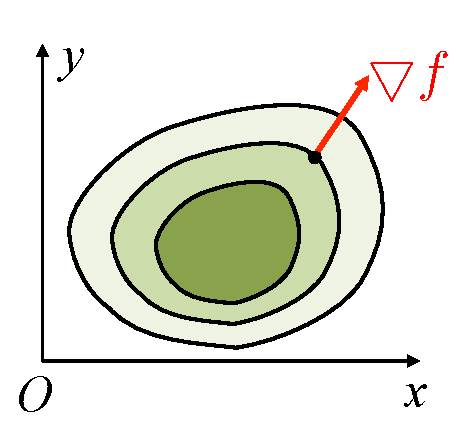
\includegraphics{./images/ch10/fxyc.pdf}}
				
				\pause {\bb 等值(高)线:}$f(x,y)=c$\pause 
			\end{center}
		\column{.5\textwidth}
			\begin{center}
				\resizebox{!}{4.5cm}{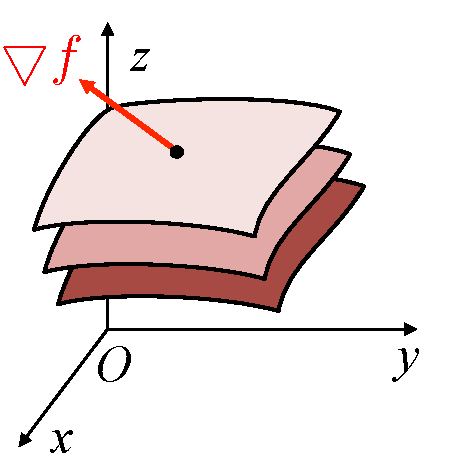
\includegraphics{./images/ch10/fxyzc.pdf}}
				
				\pause {\bb 等值面:}$f(x,y,z)=c$
			\end{center}
	\end{columns}	
\end{frame}

\section{方向导数与梯度的应用}

\begin{frame}{方向导数与梯度的应用}
	\linespread{1.2}\pause 
	\begin{block}{{\bf 定理10.4.2}\hfill}
		设$f(\bm{x})$在$\bm{x}_0$可微,$\bm{u}$为非零向量,
		若$D_{\bm{u}}f(\bm{x}_0)>0$,则$\bm{u}$为
		  $f(\bm{x})$在$\bm{x}_0$处的一个{\bb 上升方向};\pause 
		  反之为一个{\bb 下降方向}。
% 		\begin{enumerate}
% 		  \item 若$D_{\bm{u}}f(\bm{x}_0)>0$,则$\bm{u}$为
% 		  $f(\bm{x})$在$\bm{x}_0$处的一个{\bb 上升方向};
% 		  \item 反之为一个{\bb 下降方向}。
% 		\end{enumerate}
	\end{block}\pause 
	\begin{block}{{\bf 推论}\hfill}
% 		\begin{enumerate}
% 		  \item 
		  若$\bm{x}_0$为可微函数$f(\bm{x})$的一个{\bb 局部最小(大)值}点,
		  则对任意$\bm{u}\ne 0$,$D_{\bm{u}}f(\bm{x}_0)=0$。
% 		\end{enumerate}
	\end{block}
	\begin{itemize}\pause 
	  \item Fermat引理的推广
	\end{itemize}
\end{frame}

\section{Hessian矩阵}

\begin{frame}{Hessian矩阵}
	\linespread{1.2}\pause 
	\begin{block}{{\bf 定义}\hfill}
		设$f(\bm{x})\,(\bm{x}=(x_1,x_2,\ldots,x_n))$的所有二阶偏导数连续\pause 
		$$H=\left[\begin{array}{cccc}
			\df{\p^2 f}{\p x_1^2} & \df{\p^2 f}{\p x_1\p x_2} & \ldots & \df{\p^2
			f}{\p x_1\p x_n}\\[10pt]
			\df{\p^2 f}{\p x_2\p x_1} & \df{\p^2 f}{\p x_2^2} & \ldots & \df{\p^2
			f}{\p x_2\p x_n}\\[10pt]
			\ldots & \ldots & \ldots & \ldots\\[6pt]
			\df{\p^2 f}{\p x_n\p x_1} & \df{\p^2 f}{\p x_n\p x_2} & \ldots & \df{\p^2
			f}{\p x_n^2}
			\end{array}\right]
		\pause =\bigtriangledown^2 f(\bm{x})$$
	\end{block}
\end{frame}

\begin{frame}
	\linespread{1.2}
	\begin{exampleblock}{{\bf 例4}\hfill}
		计算$f(x,y)=x^4+xy+(1+y)^2$的Hessian矩阵。
	\end{exampleblock}
	\bigskip\pause 
	\begin{exampleblock}{{\bf 例5}\hfill}
		设$\bm{a},\bm{b},\bm{x}\in\mathbb{R}^n,\bm{Q}
		\in\mathbb{R}^{n\times n},\bm{Q}=\bm{Q}^T,c\in\mathbb{R}$,求以下函数的梯度与Hessian矩阵:
		\begin{enumerate}
		  \item $f(\bm{x})=\bm{b}\bm{x}^{T}+c$
		  \item $g(\bm{x})=\df 12\bm{x}\bm{Q}\bm{x}^T+\bm{b}\bm{x}^{T}+c$
		\end{enumerate}
	\end{exampleblock}
\end{frame}

\section{多元Taylor公式}

\begin{frame}{多元Taylor公式}
	\linespread{1.2}\pause 
	\begin{block}{{\bf 定理10.4.4}\hfill}
		设$n$元函数$f(\bm{x})$在$\bm{x}_0$的某邻域内二阶偏导数连续,\pause 
		则:对该领域内任意点$\bm{x}$,\pause 存在$\theta\in(0,1)$,\pause 使得
		\begin{eqnarray*}
			f(\bm{x}) & = & f(\bm{x}_0)+\bigtriangledown f(\bm{x}_0)(\bm{x}-\bm{x}_0)^T\\
			& & + \df 12(\bm{x}-\bm{x}_0)\bigtriangledown^2
			f(\bm{x}_0+\theta(\bm{x}-\bm{x}_0))(\bm{x}-\bm{x}_0)^T
 		\end{eqnarray*}\pause 
 		即:{\bb $f(\bm{x})$在$\bm{x}_0$处带Lagrange余项的Taylor公式}
	\end{block}
\end{frame}

\begin{frame}
	\linespread{1.2}
	{\bb $f(\bm{x})$在$\bm{x}_0$处带Peano余项的Taylor公式:}\pause 
	\begin{eqnarray*}
			f(\bm{x}) & = & f(\bm{x}_0)+\bigtriangledown f(\bm{x}_0)(\bm{x}-\bm{x}_0)^T\\
			& & + \df 12(\bm{x}-\bm{x}_0)\bigtriangledown^2
			f(\bm{x}_0)(\bm{x}-\bm{x}_0)^T+\circ(|\bm{x}-\bm{x}_0|^2)
 		\end{eqnarray*}\pause 
	\begin{exampleblock}{{\bf 例6}\hfill}
		求$f(x,y)=x^4+xy+(1+y)^2$在原点处带Peano余项的一阶及二阶Taylor公式。
	\end{exampleblock}
\end{frame}

\begin{frame}[<+->]{小结}
	\linespread{1.5}
	\begin{enumerate}
	  \item {\bf 方向导数与梯度}
	  $$D_{\bm{u}}f=\bigtriangledown f\cdot\bm{e_u}$$
	  \vspace{-2em}
	  \begin{itemize}
	    \item 梯度:法线方向
	  \end{itemize}
	  \item {\bf Hessian矩阵与Taylor公式}
	  \begin{itemize}
	    \item $\bigtriangledown^2 f$:多元函数的二阶导数
	    \item 了解二元的二阶Taylor公式
	  \end{itemize}
	\end{enumerate}
\end{frame}

%=====================================
 
% \begin{frame}{title}
% 	\linespread{1.2}
% 	\begin{exampleblock}{{\bf title}\hfill}
% 		123
% 	\end{exampleblock}
% \end{frame}
% 
% \begin{frame}{title}
% 	\linespread{1.2}
% 	\begin{block}{{\bf title}\hfill}
% 		123
% 	\end{block}
% \end{frame}